\documentclass{standalone}
\usepackage{tikz}
\usetikzlibrary{patterns, positioning}
\usetikzlibrary{shapes.misc}
\usepackage[outline]{contour}
\contourlength{1.5pt} 
\usepackage[sfdefault]{ClearSans} %% option 'sfdefault' activates Clear Sans as the default text font
\usepackage[T1]{fontenc}

\begin{document}
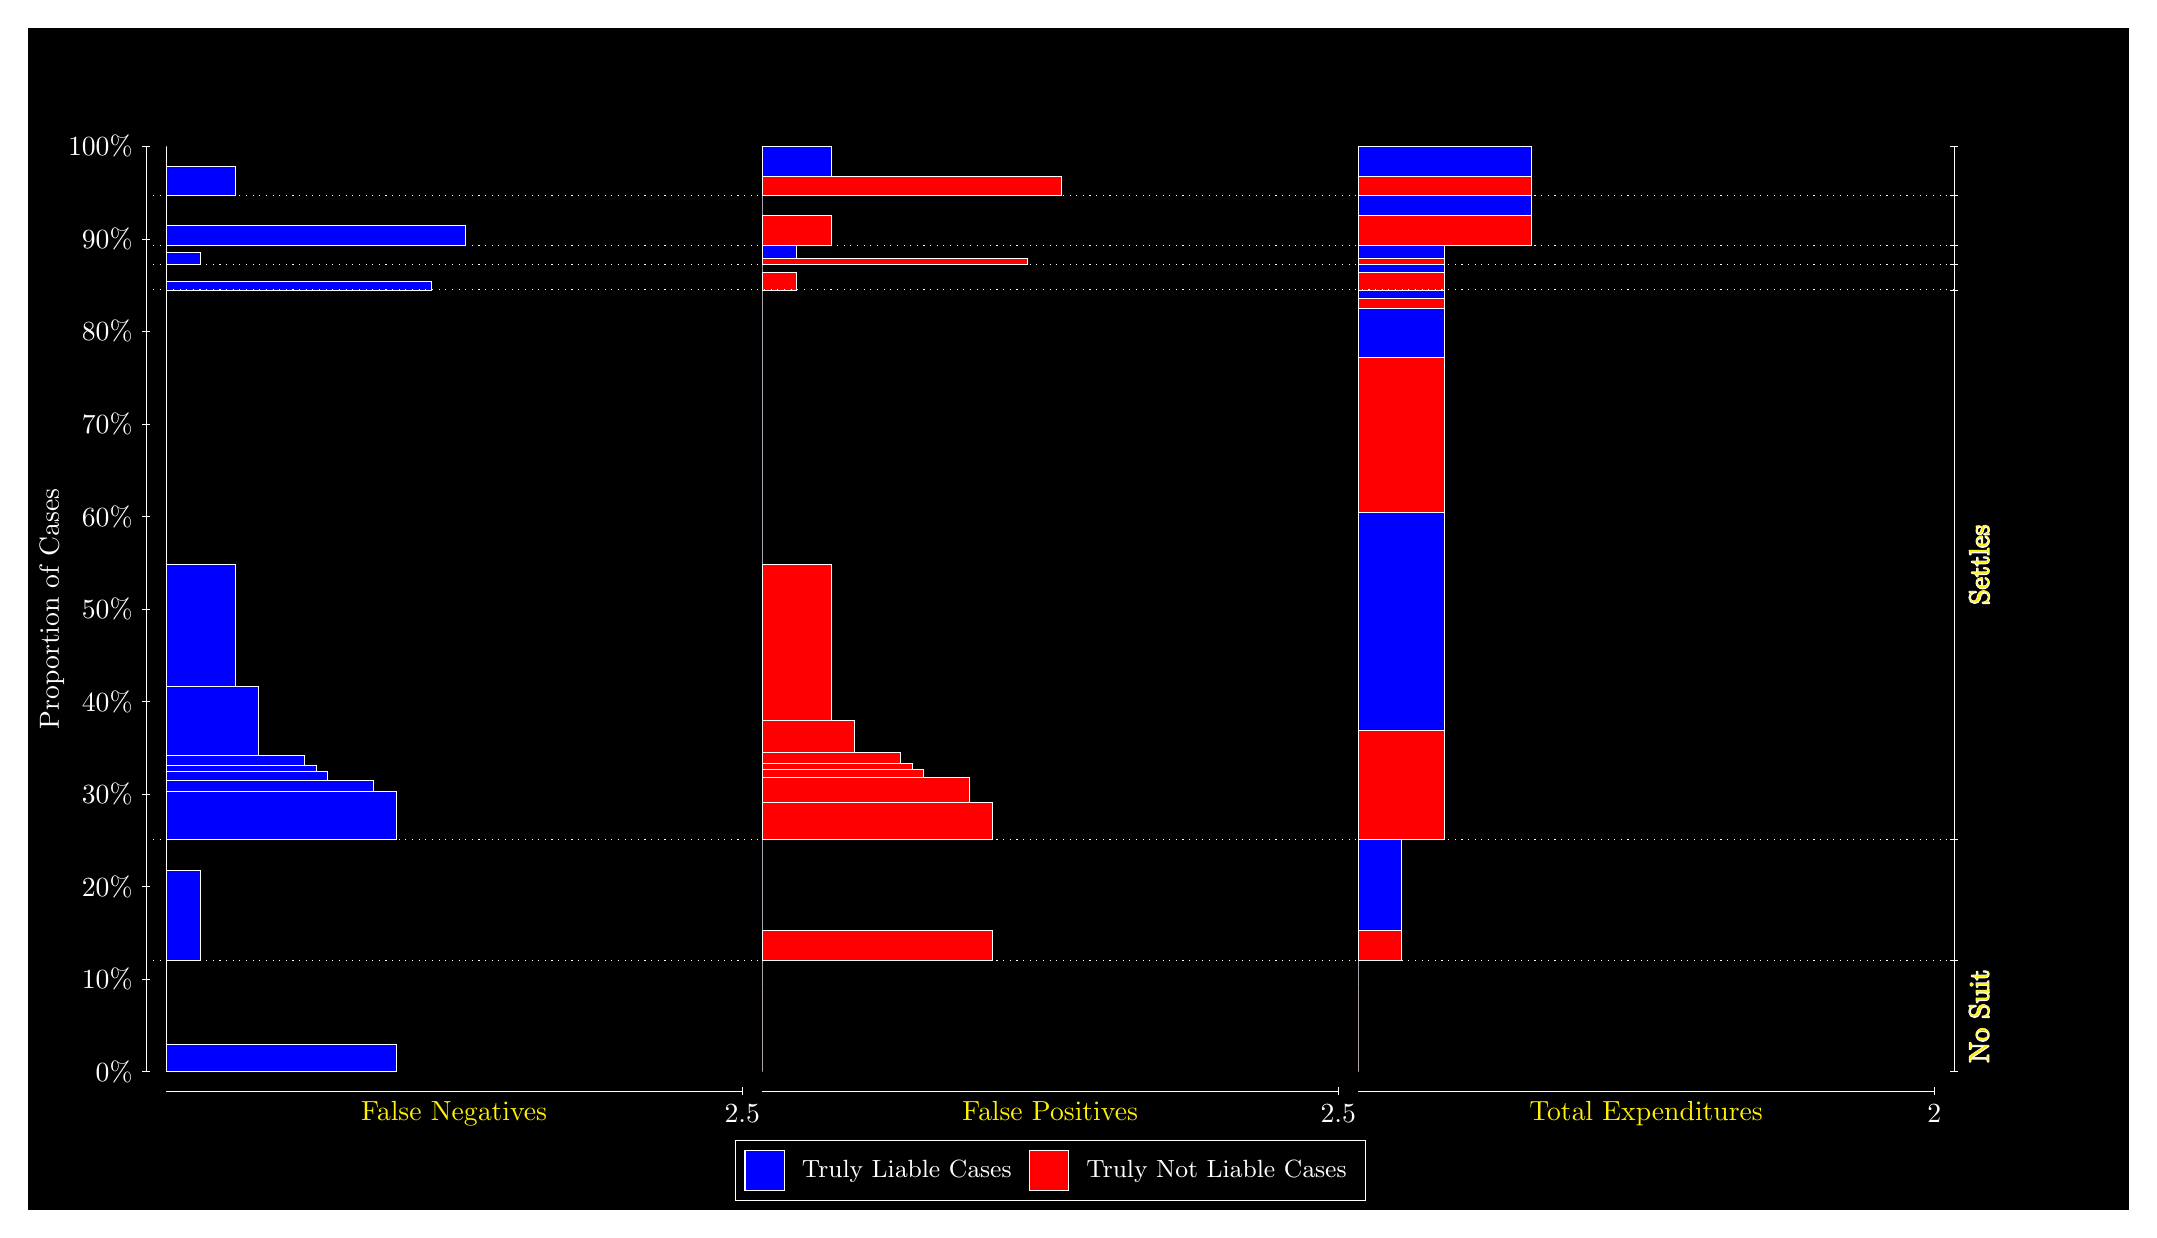
\begin{tikzpicture}
\draw[fill=black] (0,0) rectangle (26.667,15);
\draw[white, very thin] (1.5,1.75) -- (1.5,13.5);
\node[rotate=90, text=white, anchor=center] at (0.3, 7.625) {Proportion of Cases};
\draw[white, very thin] (1.45,1.75) -- (1.55,1.75);
\node[text=white, anchor=east] at (1.45, 1.75) {0\%};
\draw[white, very thin] (1.45,2.925) -- (1.55,2.925);
\node[text=white, anchor=east] at (1.45, 2.925) {10\%};
\draw[white, very thin] (1.45,4.1) -- (1.55,4.1);
\node[text=white, anchor=east] at (1.45, 4.1) {20\%};
\draw[white, very thin] (1.45,5.275) -- (1.55,5.275);
\node[text=white, anchor=east] at (1.45, 5.275) {30\%};
\draw[white, very thin] (1.45,6.45) -- (1.55,6.45);
\node[text=white, anchor=east] at (1.45, 6.45) {40\%};
\draw[white, very thin] (1.45,7.625) -- (1.55,7.625);
\node[text=white, anchor=east] at (1.45, 7.625) {50\%};
\draw[white, very thin] (1.45,8.8) -- (1.55,8.8);
\node[text=white, anchor=east] at (1.45, 8.8) {60\%};
\draw[white, very thin] (1.45,9.975) -- (1.55,9.975);
\node[text=white, anchor=east] at (1.45, 9.975) {70\%};
\draw[white, very thin] (1.45,11.15) -- (1.55,11.15);
\node[text=white, anchor=east] at (1.45, 11.15) {80\%};
\draw[white, very thin] (1.45,12.325) -- (1.55,12.325);
\node[text=white, anchor=east] at (1.45, 12.325) {90\%};
\draw[white, very thin] (1.45,13.5) -- (1.55,13.5);
\node[text=white, anchor=east] at (1.45, 13.5) {100\%};

\draw[white, very thin] (24.457,1.75) -- (24.457,13.5);
\draw[white, very thin] (24.407,1.75) -- (24.507,1.75);
\node[anchor=west] at (24.407, 1.75) {};
\draw[white, very thin] (24.407,3.1584) -- (24.507,3.1584);
\node[anchor=west] at (24.407, 3.1584) {};
\draw[white, very thin] (24.407,4.6952) -- (24.507,4.6952);
\node[anchor=west] at (24.407, 4.6952) {};
\draw[white, very thin] (24.407,11.678) -- (24.507,11.678);
\node[anchor=west] at (24.407, 11.678) {};
\draw[white, very thin] (24.407,12) -- (24.507,12);
\node[anchor=west] at (24.407, 12) {};
\draw[white, very thin] (24.407,12.241) -- (24.507,12.241);
\node[anchor=west] at (24.407, 12.241) {};
\draw[white, very thin] (24.407,12.872) -- (24.507,12.872);
\node[anchor=west] at (24.407, 12.872) {};
\draw[white, very thin] (24.407,13.5) -- (24.507,13.5);
\node[anchor=west] at (24.407, 13.5) {};

\draw[white, very thin, fill=blue] (1.75,1.75) rectangle (4.6775,2.092);
\draw[white, very thin, fill=red] (1.75,2.092) rectangle (1.75,3.1584);
\draw[white, very thin, fill=blue] (1.75,3.1584) rectangle (2.1891,4.3082);
\draw[white, very thin, fill=red] (1.75,4.3082) rectangle (1.75,4.6952);
\draw[white, very thin, fill=blue] (1.75,4.6952) rectangle (4.6775,5.3149);
\draw[white, very thin, fill=blue] (1.75,5.3149) rectangle (4.3848,5.4544);
\draw[white, very thin, fill=blue] (1.75,5.4544) rectangle (3.7993,5.5598);
\draw[white, very thin, fill=blue] (1.75,5.5598) rectangle (3.6529,5.6373);
\draw[white, very thin, fill=blue] (1.75,5.6373) rectangle (3.5065,5.7672);
\draw[white, very thin, fill=blue] (1.75,5.7672) rectangle (2.921,6.6367);
\draw[white, very thin, fill=blue] (1.75,6.6367) rectangle (2.6283,8.1876);
\draw[white, very thin, fill=red] (1.75,8.1876) rectangle (1.75,11.678);
\draw[white, very thin, fill=blue] (1.75,11.678) rectangle (5.1167,11.783);
\draw[white, very thin, fill=red] (1.75,11.783) rectangle (1.75,12);
\draw[white, very thin, fill=blue] (1.75,12) rectangle (2.1891,12.157);
\draw[white, very thin, fill=red] (1.75,12.157) rectangle (1.75,12.241);
\draw[white, very thin, fill=blue] (1.75,12.241) rectangle (5.5558,12.492);
\draw[white, very thin, fill=red] (1.75,12.492) rectangle (1.75,12.872);
\draw[white, very thin, fill=blue] (1.75,12.872) rectangle (2.6283,13.249);
\draw[white, very thin, fill=red] (1.75,13.249) rectangle (1.75,13.5);
\draw[white, very thin, fill=red] (9.3189,1.75) rectangle (9.3189,2.8164);
\draw[white, very thin, fill=blue] (9.3189,2.8164) rectangle (9.3189,3.1584);
\draw[white, very thin, fill=red] (9.3189,3.1584) rectangle (12.246,3.5454);
\draw[white, very thin, fill=blue] (9.3189,3.5454) rectangle (9.3189,4.6952);
\draw[white, very thin, fill=red] (9.3189,4.6952) rectangle (12.246,5.1753);
\draw[white, very thin, fill=red] (9.3189,5.1753) rectangle (11.954,5.4854);
\draw[white, very thin, fill=red] (9.3189,5.4854) rectangle (11.368,5.5908);
\draw[white, very thin, fill=red] (9.3189,5.5908) rectangle (11.222,5.6683);
\draw[white, very thin, fill=red] (9.3189,5.6683) rectangle (11.075,5.7982);
\draw[white, very thin, fill=red] (9.3189,5.7982) rectangle (10.49,6.2166);
\draw[white, very thin, fill=red] (9.3189,6.2166) rectangle (10.197,8.186);
\draw[white, very thin, fill=blue] (9.3189,8.186) rectangle (9.3189,11.678);
\draw[white, very thin, fill=red] (9.3189,11.678) rectangle (9.758,11.895);
\draw[white, very thin, fill=blue] (9.3189,11.895) rectangle (9.3189,12);
\draw[white, very thin, fill=red] (9.3189,12) rectangle (12.686,12.083);
\draw[white, very thin, fill=blue] (9.3189,12.083) rectangle (9.758,12.241);
\draw[white, very thin, fill=red] (9.3189,12.241) rectangle (10.197,12.621);
\draw[white, very thin, fill=blue] (9.3189,12.621) rectangle (9.3189,12.872);
\draw[white, very thin, fill=red] (9.3189,12.872) rectangle (13.125,13.123);
\draw[white, very thin, fill=blue] (9.3189,13.123) rectangle (10.197,13.5);
\draw[white, very thin, fill=red] (16.888,1.75) rectangle (16.888,2.8164);
\draw[white, very thin, fill=blue] (16.888,2.8164) rectangle (16.888,3.1584);
\draw[white, very thin, fill=red] (16.888,3.1584) rectangle (17.437,3.5454);
\draw[white, very thin, fill=blue] (16.888,3.5454) rectangle (17.437,4.6952);
\draw[white, very thin, fill=red] (16.888,4.6952) rectangle (17.986,6.0867);
\draw[white, very thin, fill=blue] (16.888,6.0867) rectangle (17.986,8.8541);
\draw[white, very thin, fill=red] (16.888,8.8541) rectangle (17.986,10.823);
\draw[white, very thin, fill=blue] (16.888,10.823) rectangle (17.986,11.443);
\draw[white, very thin, fill=red] (16.888,11.443) rectangle (17.986,11.573);
\draw[white, very thin, fill=blue] (16.888,11.573) rectangle (17.986,11.678);
\draw[white, very thin, fill=red] (16.888,11.678) rectangle (17.986,11.895);
\draw[white, very thin, fill=blue] (16.888,11.895) rectangle (17.986,12);
\draw[white, very thin, fill=red] (16.888,12) rectangle (17.986,12.083);
\draw[white, very thin, fill=blue] (16.888,12.083) rectangle (17.986,12.241);
\draw[white, very thin, fill=red] (16.888,12.241) rectangle (19.083,12.621);
\draw[white, very thin, fill=blue] (16.888,12.621) rectangle (19.083,12.872);
\draw[white, very thin, fill=red] (16.888,12.872) rectangle (19.083,13.123);
\draw[white, very thin, fill=blue] (16.888,13.123) rectangle (19.083,13.5);
\draw[white, dotted] (1.5,3.1584) -- (24.457,3.1584);
\draw[white, dotted] (1.5,4.6952) -- (24.457,4.6952);
\draw[white, dotted] (1.5,11.678) -- (24.457,11.678);
\draw[white, dotted] (1.5,12) -- (24.457,12);
\draw[white, dotted] (1.5,12.241) -- (24.457,12.241);
\draw[white, dotted] (1.5,12.872) -- (24.457,12.872);
\draw[white, very thin] (1.75,1.5) -- (9.0689,1.5);
\node[text=yellow, anchor=north] at (5.4094, 1.5) {False Negatives};
\draw[white, very thin] (9.0689,1.45) -- (9.0689,1.55);
\node[text=white, anchor=north] at (9.0689, 1.45) {2.5};

\draw[white, very thin] (9.3189,1.5) -- (16.638,1.5);
\node[text=yellow, anchor=north] at (12.978, 1.5) {False Positives};
\draw[white, very thin] (16.638,1.45) -- (16.638,1.55);
\node[text=white, anchor=north] at (16.638, 1.45) {2.5};

\draw[white, very thin] (16.888,1.5) -- (24.207,1.5);
\node[text=yellow, anchor=north] at (20.547, 1.5) {Total Expenditures};
\draw[white, very thin] (24.207,1.45) -- (24.207,1.55);
\node[text=white, anchor=north] at (24.207, 1.45) {2};

\node[text=yellow, centered, rotate=90] at (24.777, 2.4542) {\contour{white}{No Suit}};

\node[text=yellow, centered, rotate=90] at (24.777, 8.1868) {\contour{white}{Settles}};





\draw (12.978300999999998,1.5) node[draw=none] (baseCoordinate) {};
\begin{scope}[align=center]
        \matrix[scale=0.5, draw=white, below=0.5cm of baseCoordinate, nodes={draw}, column sep=0.1cm]{
            \node[rectangle, draw, minimum width=0.5cm, minimum height=0.5cm, fill=blue] {}; &
            \node[draw=none, font=\small, text=white] (B) {Truly Liable Cases}; &
            \node[rectangle, draw, minimum width=0.5cm, minimum height=0.5cm, fill=red] {}; &
            \node[draw=none, font=\small, text=white] (B) {Truly Not Liable Cases}; \\
            };
\end{scope}

\end{tikzpicture}
\end{document}